\section{Resumen}
Se puede saltar hasta (aantes estaba al final pero encontre mejor explicar lo que a usted le importa al inicio y si despues queria analizar como lo hice revisar esa parte) aca y evitar todas las explicaciones previas de como lo hice y porque lo hice para ver esto.\\
Para evaluar la influencia del dominio computacional corri varias simulaciones $LeftSide=\{1,2,3\}$ y $RigthSide=\{1,2,3,4,5,6,7,8\}$, todas esas combinaciones porque esos valores, porque me di cuenta que aguas arriba tenia que convergir en un perfil similar al teorico

\begin{figure}[!ht]
    \centering
    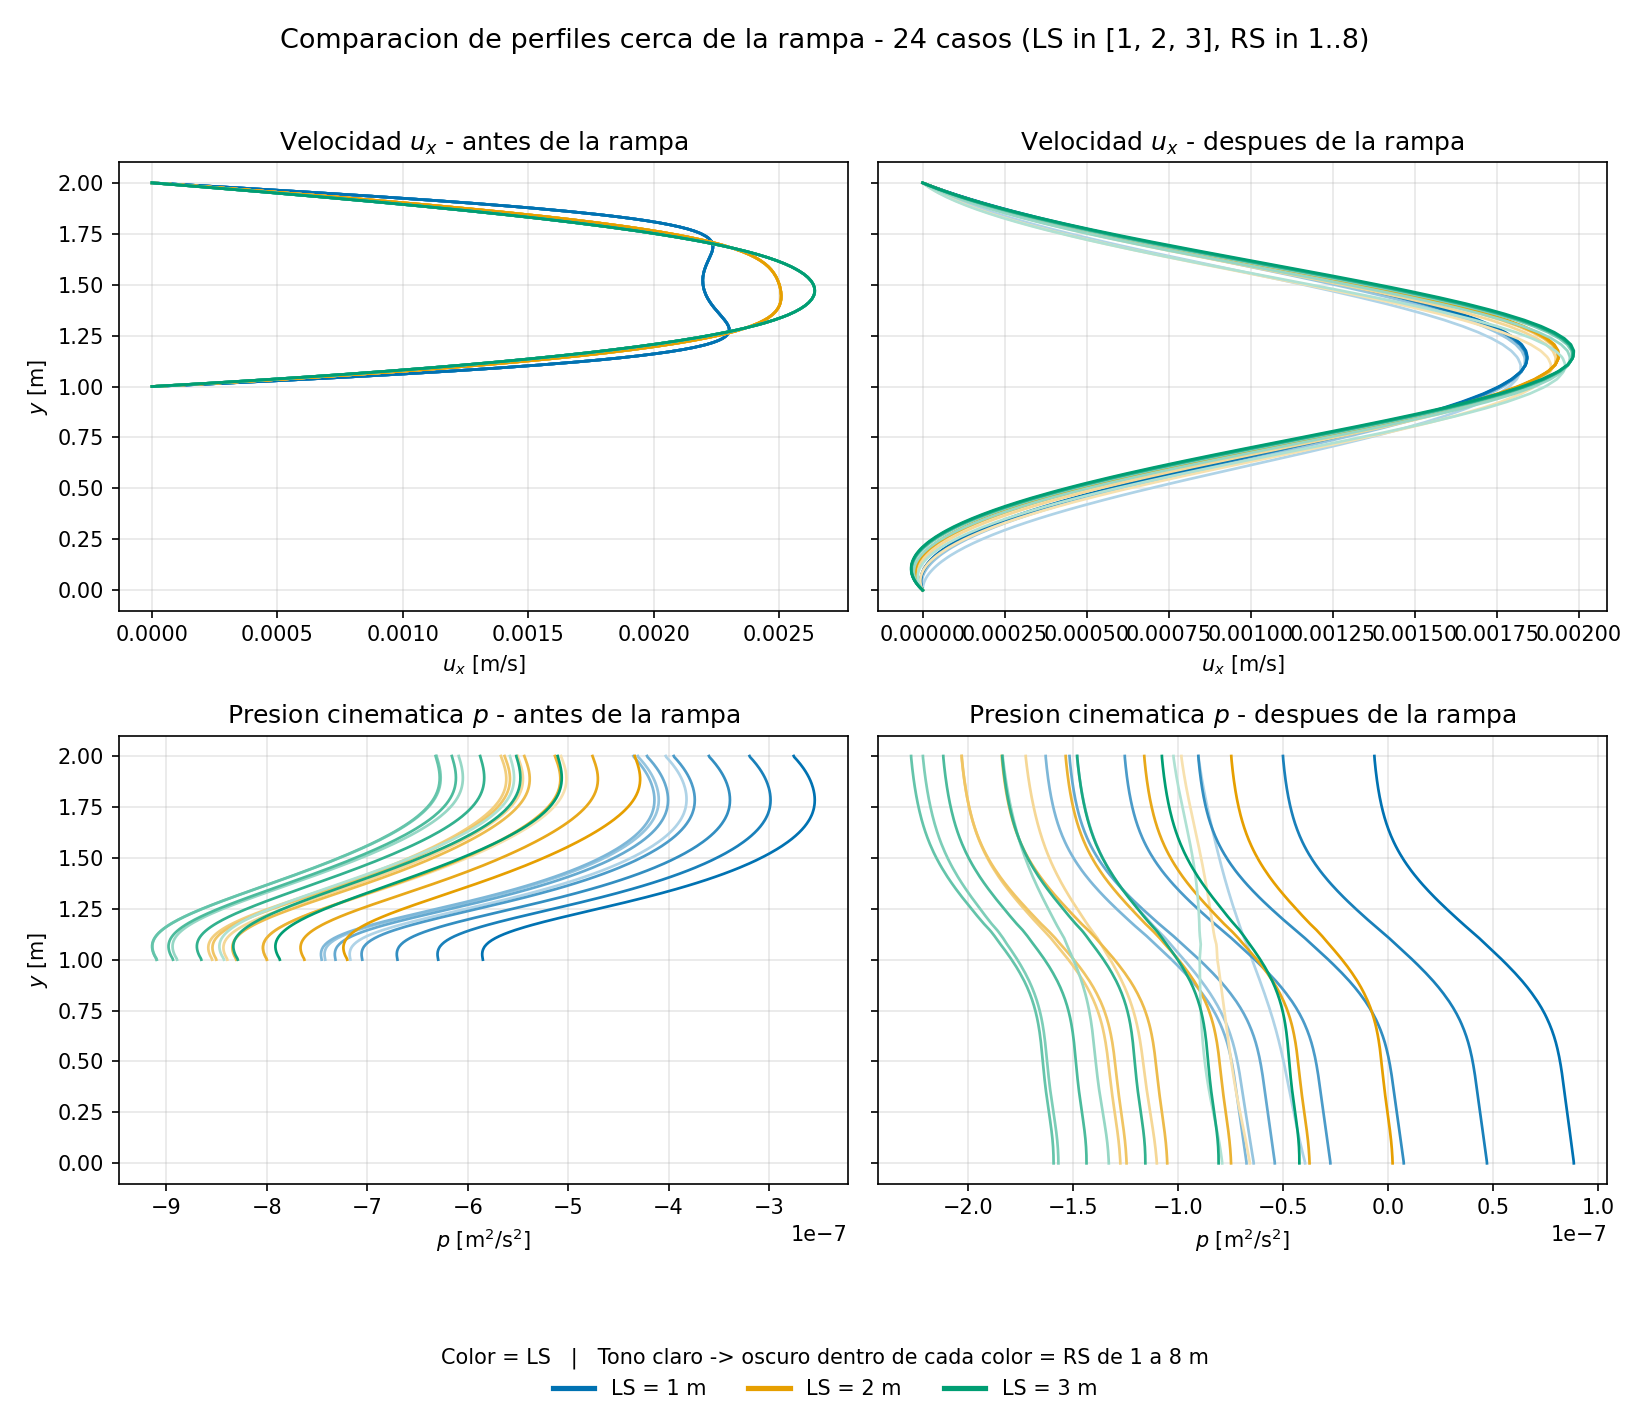
\includegraphics[width=1\linewidth]{Imagenes/T1/comparacion_rampa_24_casos.png}
    \caption{24 simulaciones, perfil de velocidad y de presion pre y post rampa}
    \label{fig:placeholder}
\end{figure}
Con esto lo que puede apreciar que la longitud post rampa no afecta a la velocidad pre rampa, pero en cambio la velocidad post rampa si depende de la longitud post rampa, lo importante de aguias arriba es para que el perfil pueda desarrollarse. En el caso de la presion me guiaria por la forma, pero no puedo guiarme mucho mas debido a que la el error residual de la simulación si bien para u es de 1e-5 por ende la exactitud de los datos no es la mejor. De igual manera para tener en cuenta, corrí con la presion a lo largo del canal (del punto medio).\\
\vspace{2cm}
\begin{figure}[!ht]
    \centering
    \caption{Presion 24 simulaciones a lo largo del canal.}
    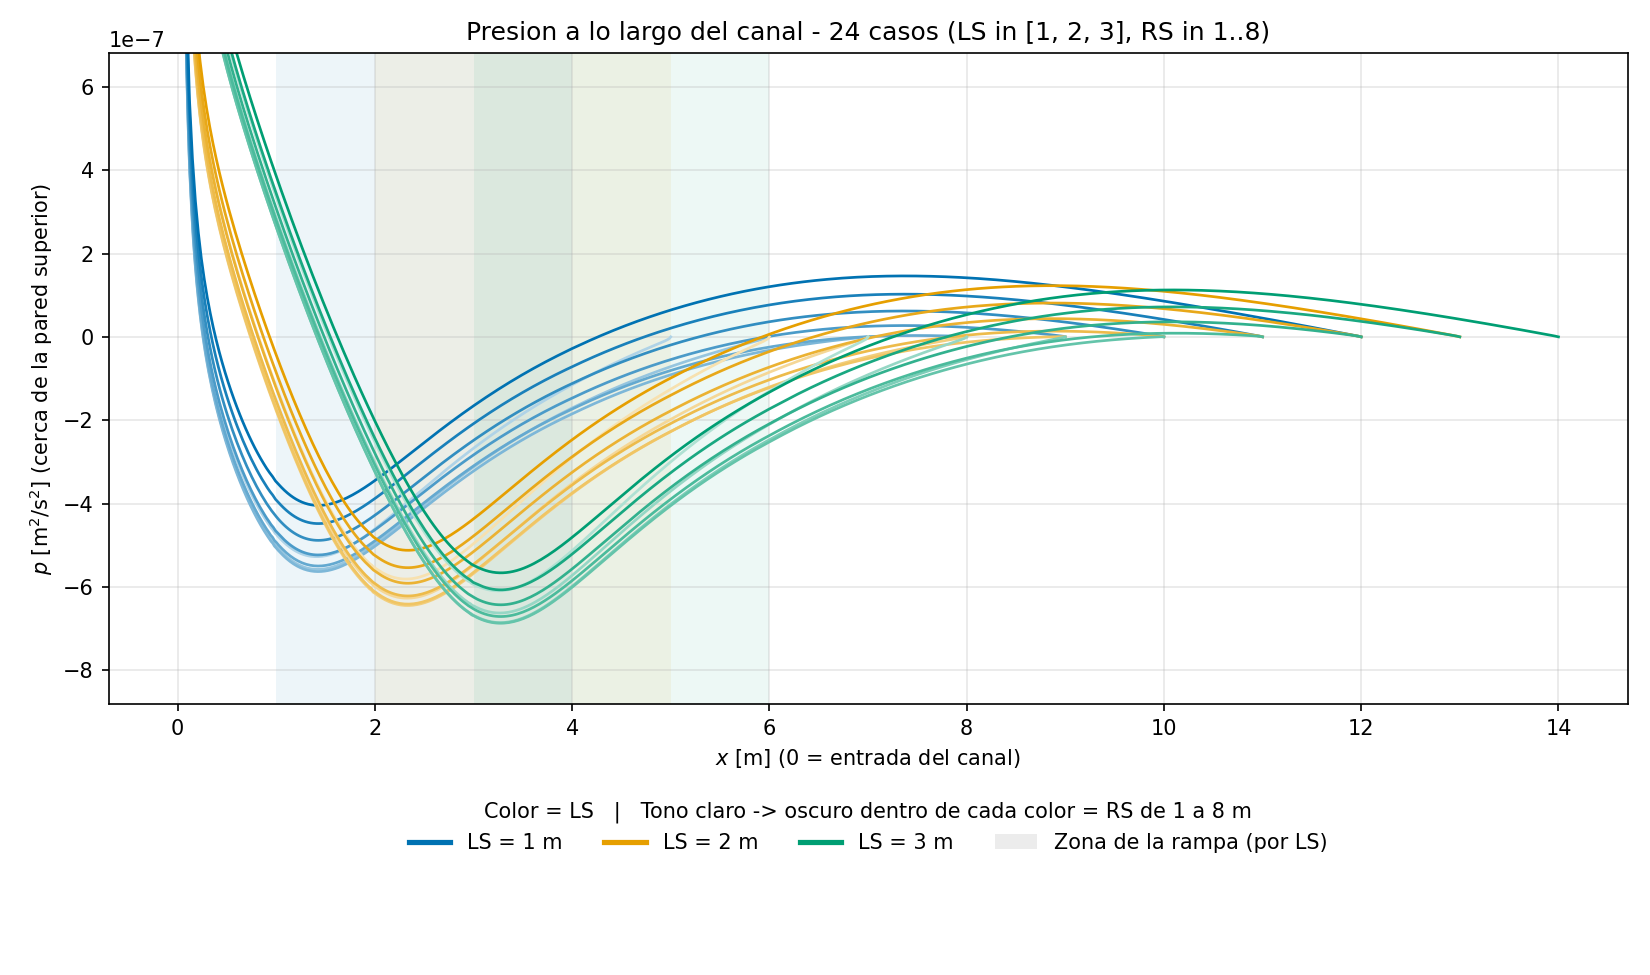
\includegraphics[width=0.8\linewidth]{Imagenes/T1/comparacion_presion_canal.png}
    \label{fig:placeholder}
\end{figure}

Aqui se puede apreciar como igual pasado el canal hay cierta recuperacion de presion donde vuelve a subir a niveles positivos y que con las simulaciones donde el RS son bajos no se puede llegar a a preciar





EL desarrollo de perfil lo podemos ver como en una simulacion general fuera de estas 24 (2.6millones de celdas con longitudes LS=10m y RS=10m) donde medi el error cuadratico respecto a la teoria Poiseuille Placas planas.
\begin{figure}[!ht]
    \centering
    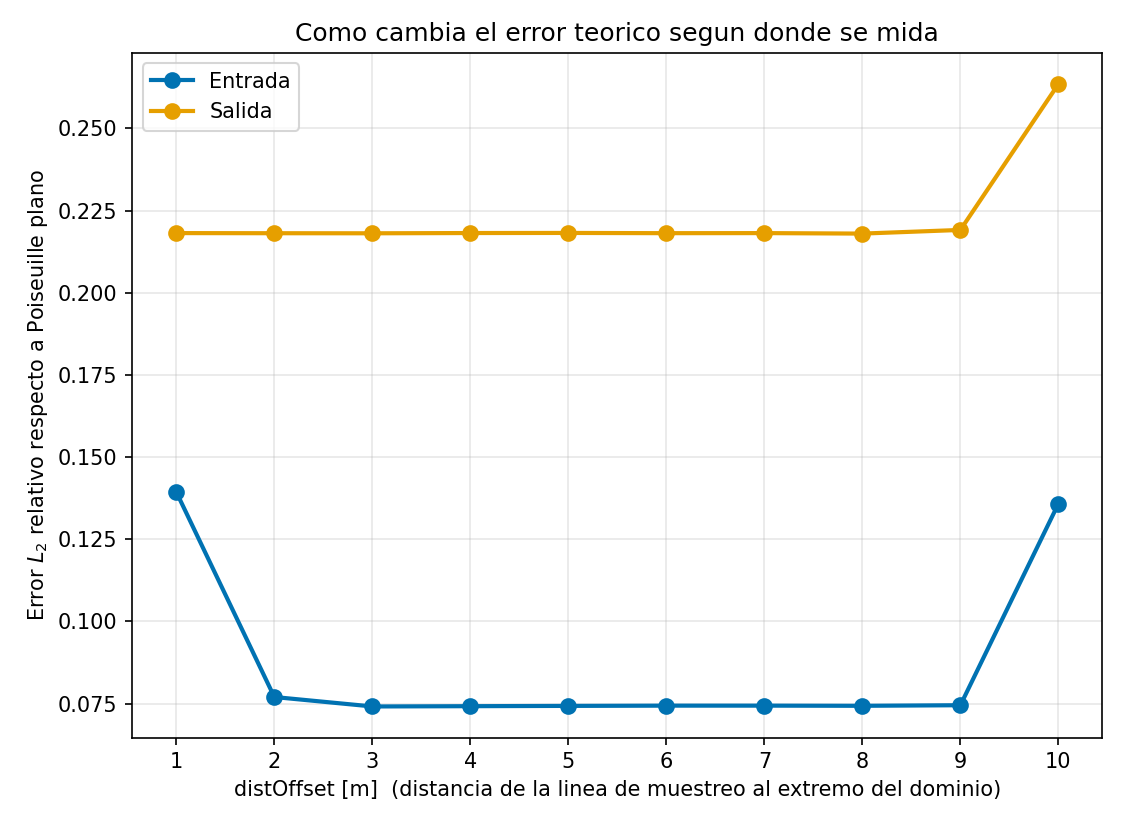
\includegraphics[width=0.5\linewidth]{Imagenes/T1/error_vs_offset.png}
    \caption{Error respecto a la distancia al extremo}
    \label{fig:placeholder}
\end{figure}
Es bueno explicar que el eje $X$ corresponde los metros post inicio o pre termino. Con esto vemos que en verdad no hay cambios en el error pasado los 2 metros post rampa (9m salida), en el caso del de entrada es porque la entrada tanto como al inicio y antes de comenzar la rampa cambia las condiciones , al inicio se coloca una velocidad uniforme pero eso no coincide con la condicion de no deslizamiento, en cambio al finalizar aguas arriba hay un gran apertura que genera un bajo de presion (bernulli)

\subsection{Zona de separacion y recuperacion de presion}
En este caso, creo que debido a el reynolds de 100 osea una velocidad baja, los efectos viscosos son mas importantes (no existe esa separacion (Ux siempre mayor a 0)), por otro lado la zona de recuperacion de la presion tambien corresponde a la zona donde la velocidad deja dispersarse (tiene compoennte en $y$) por ende una vez pasada llega a estabilizarse bastante pero como se vio antes no se llega al perfil esperado, esto puede ser debido a que en la difusion el perfil como que se dividio, generando una zona (perfil) plano, excepto en los bordes que tienen  su perfil, esto se parece mucho a la capa limite donde despues de eso el gradiente de velocidad es casi 0, lo que se llama $U_{inf}$ en mecanica de fluidos

\begin{figure}
    \centering
    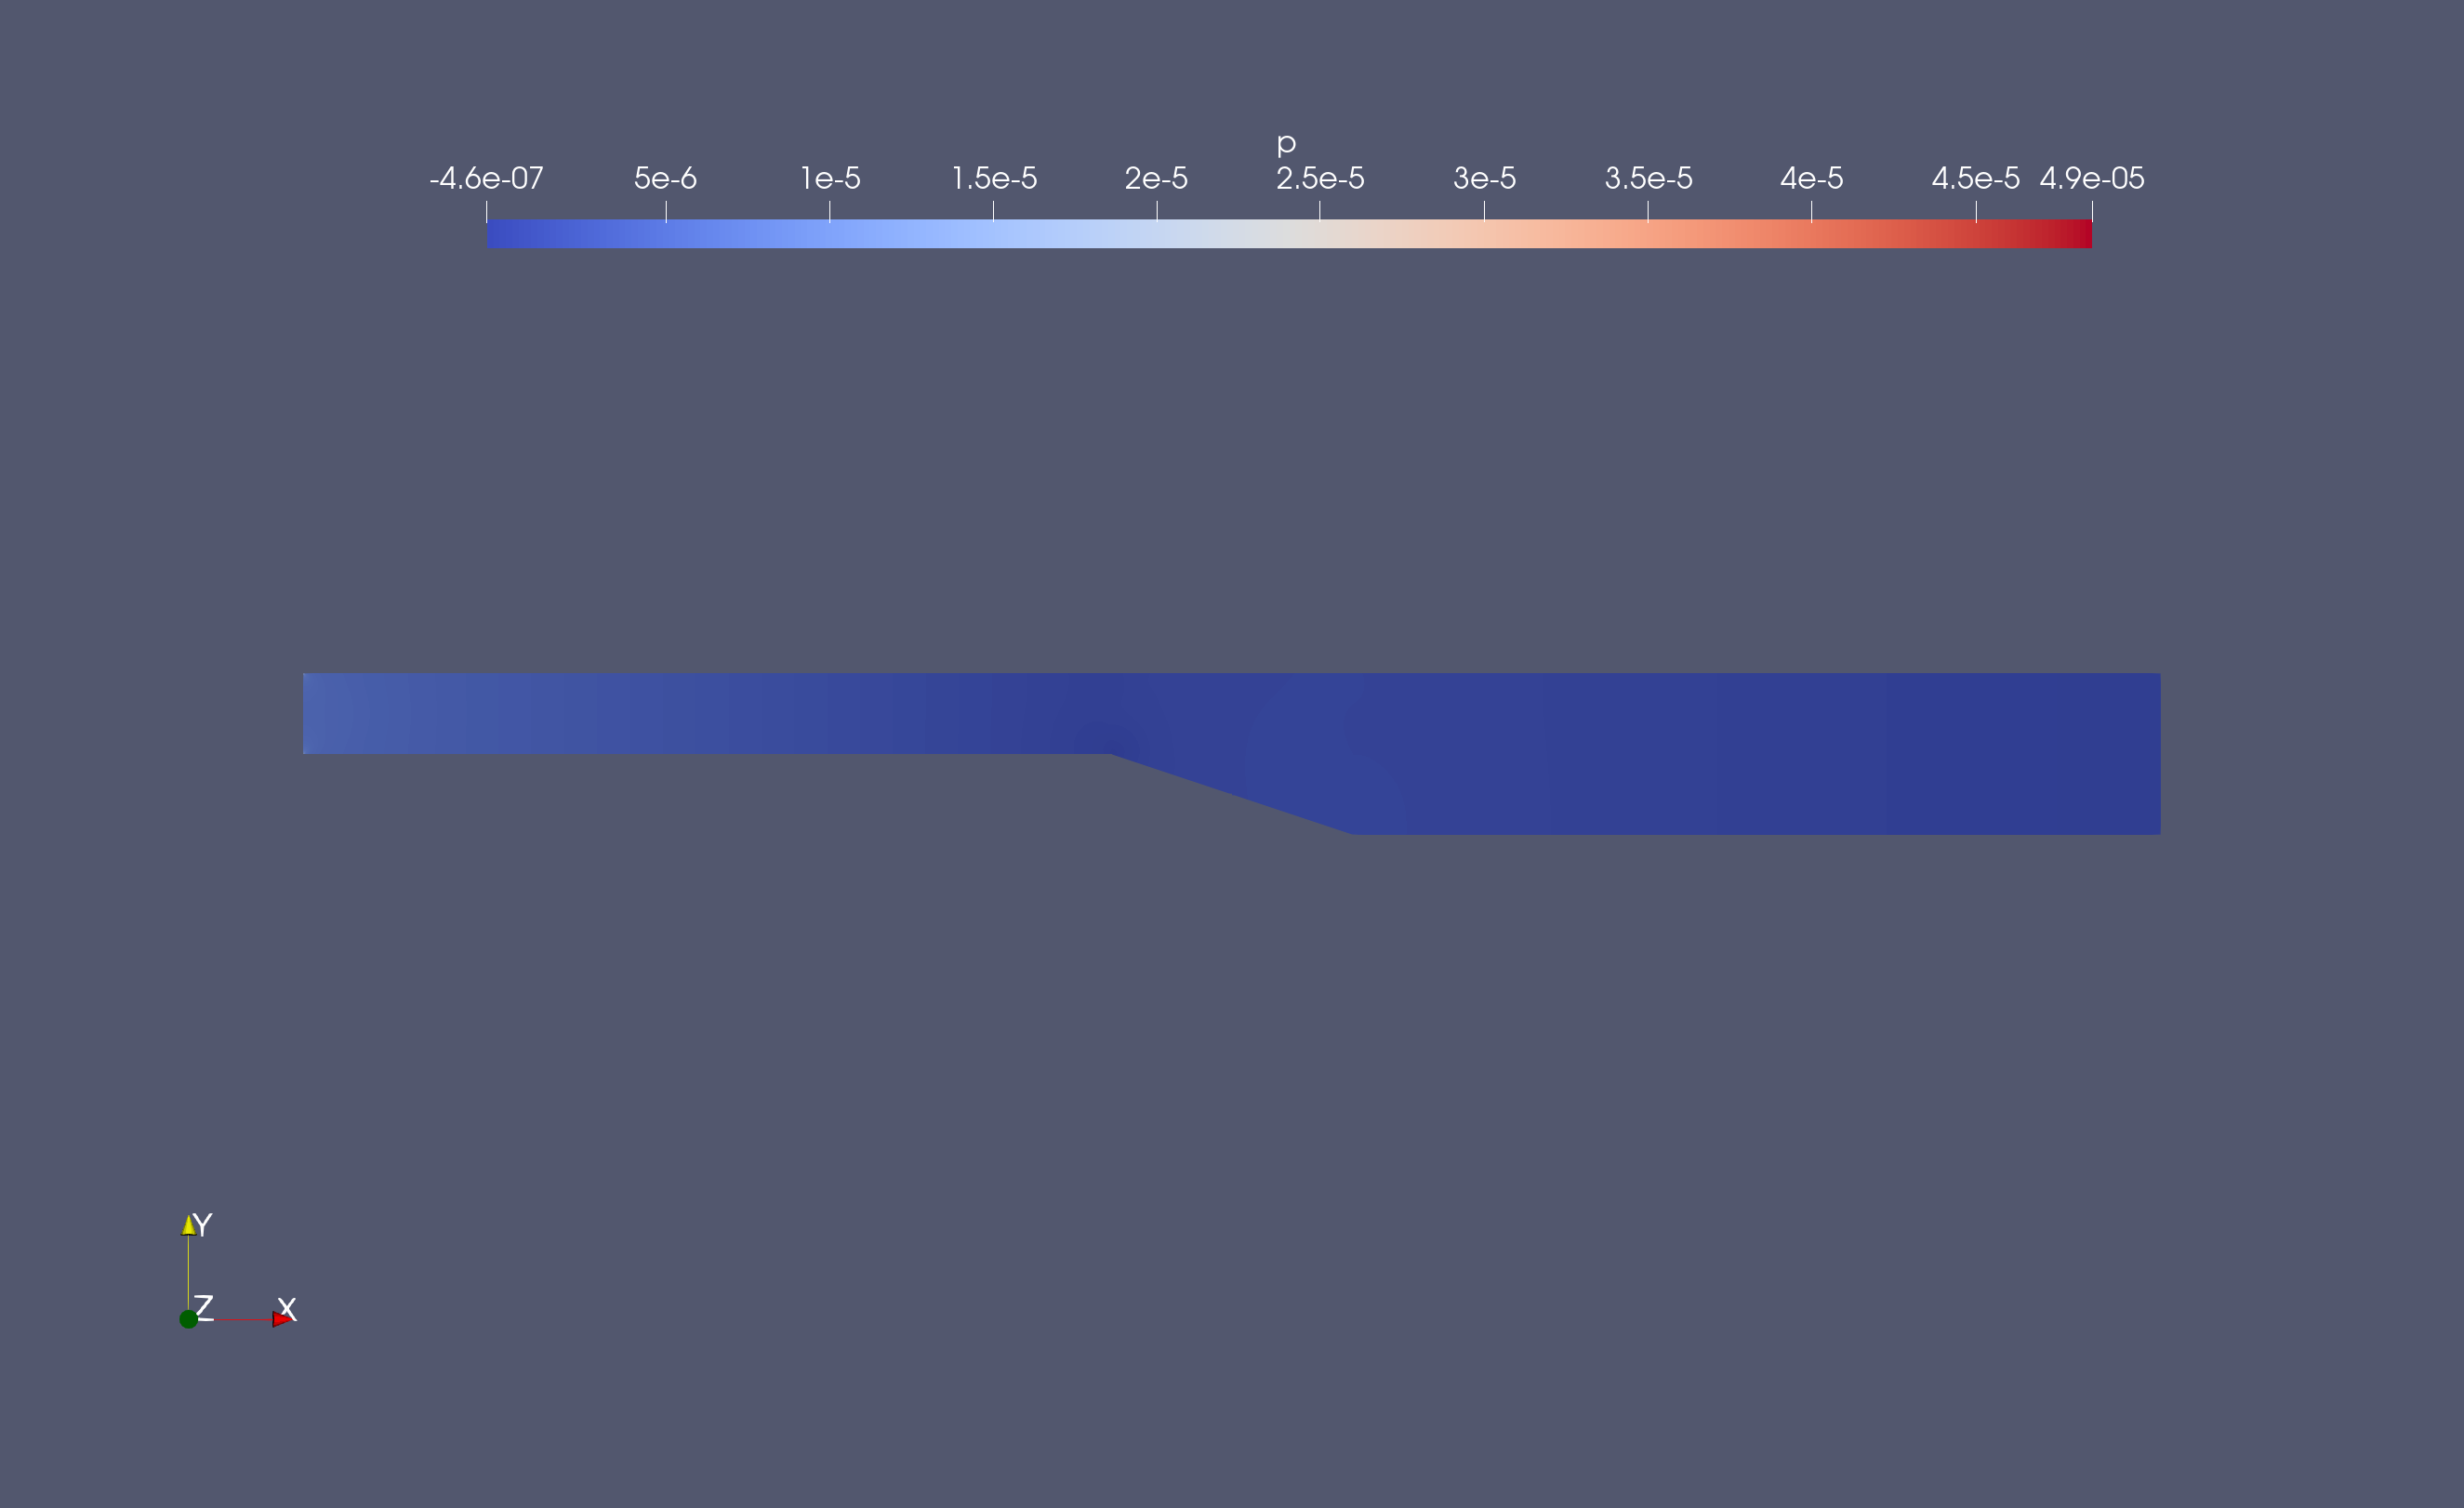
\includegraphics[width=0.5\linewidth]{Imagenes/T1/SimMillp.png}
    \caption{Presion canal simulado de 2.6millones celdas}
    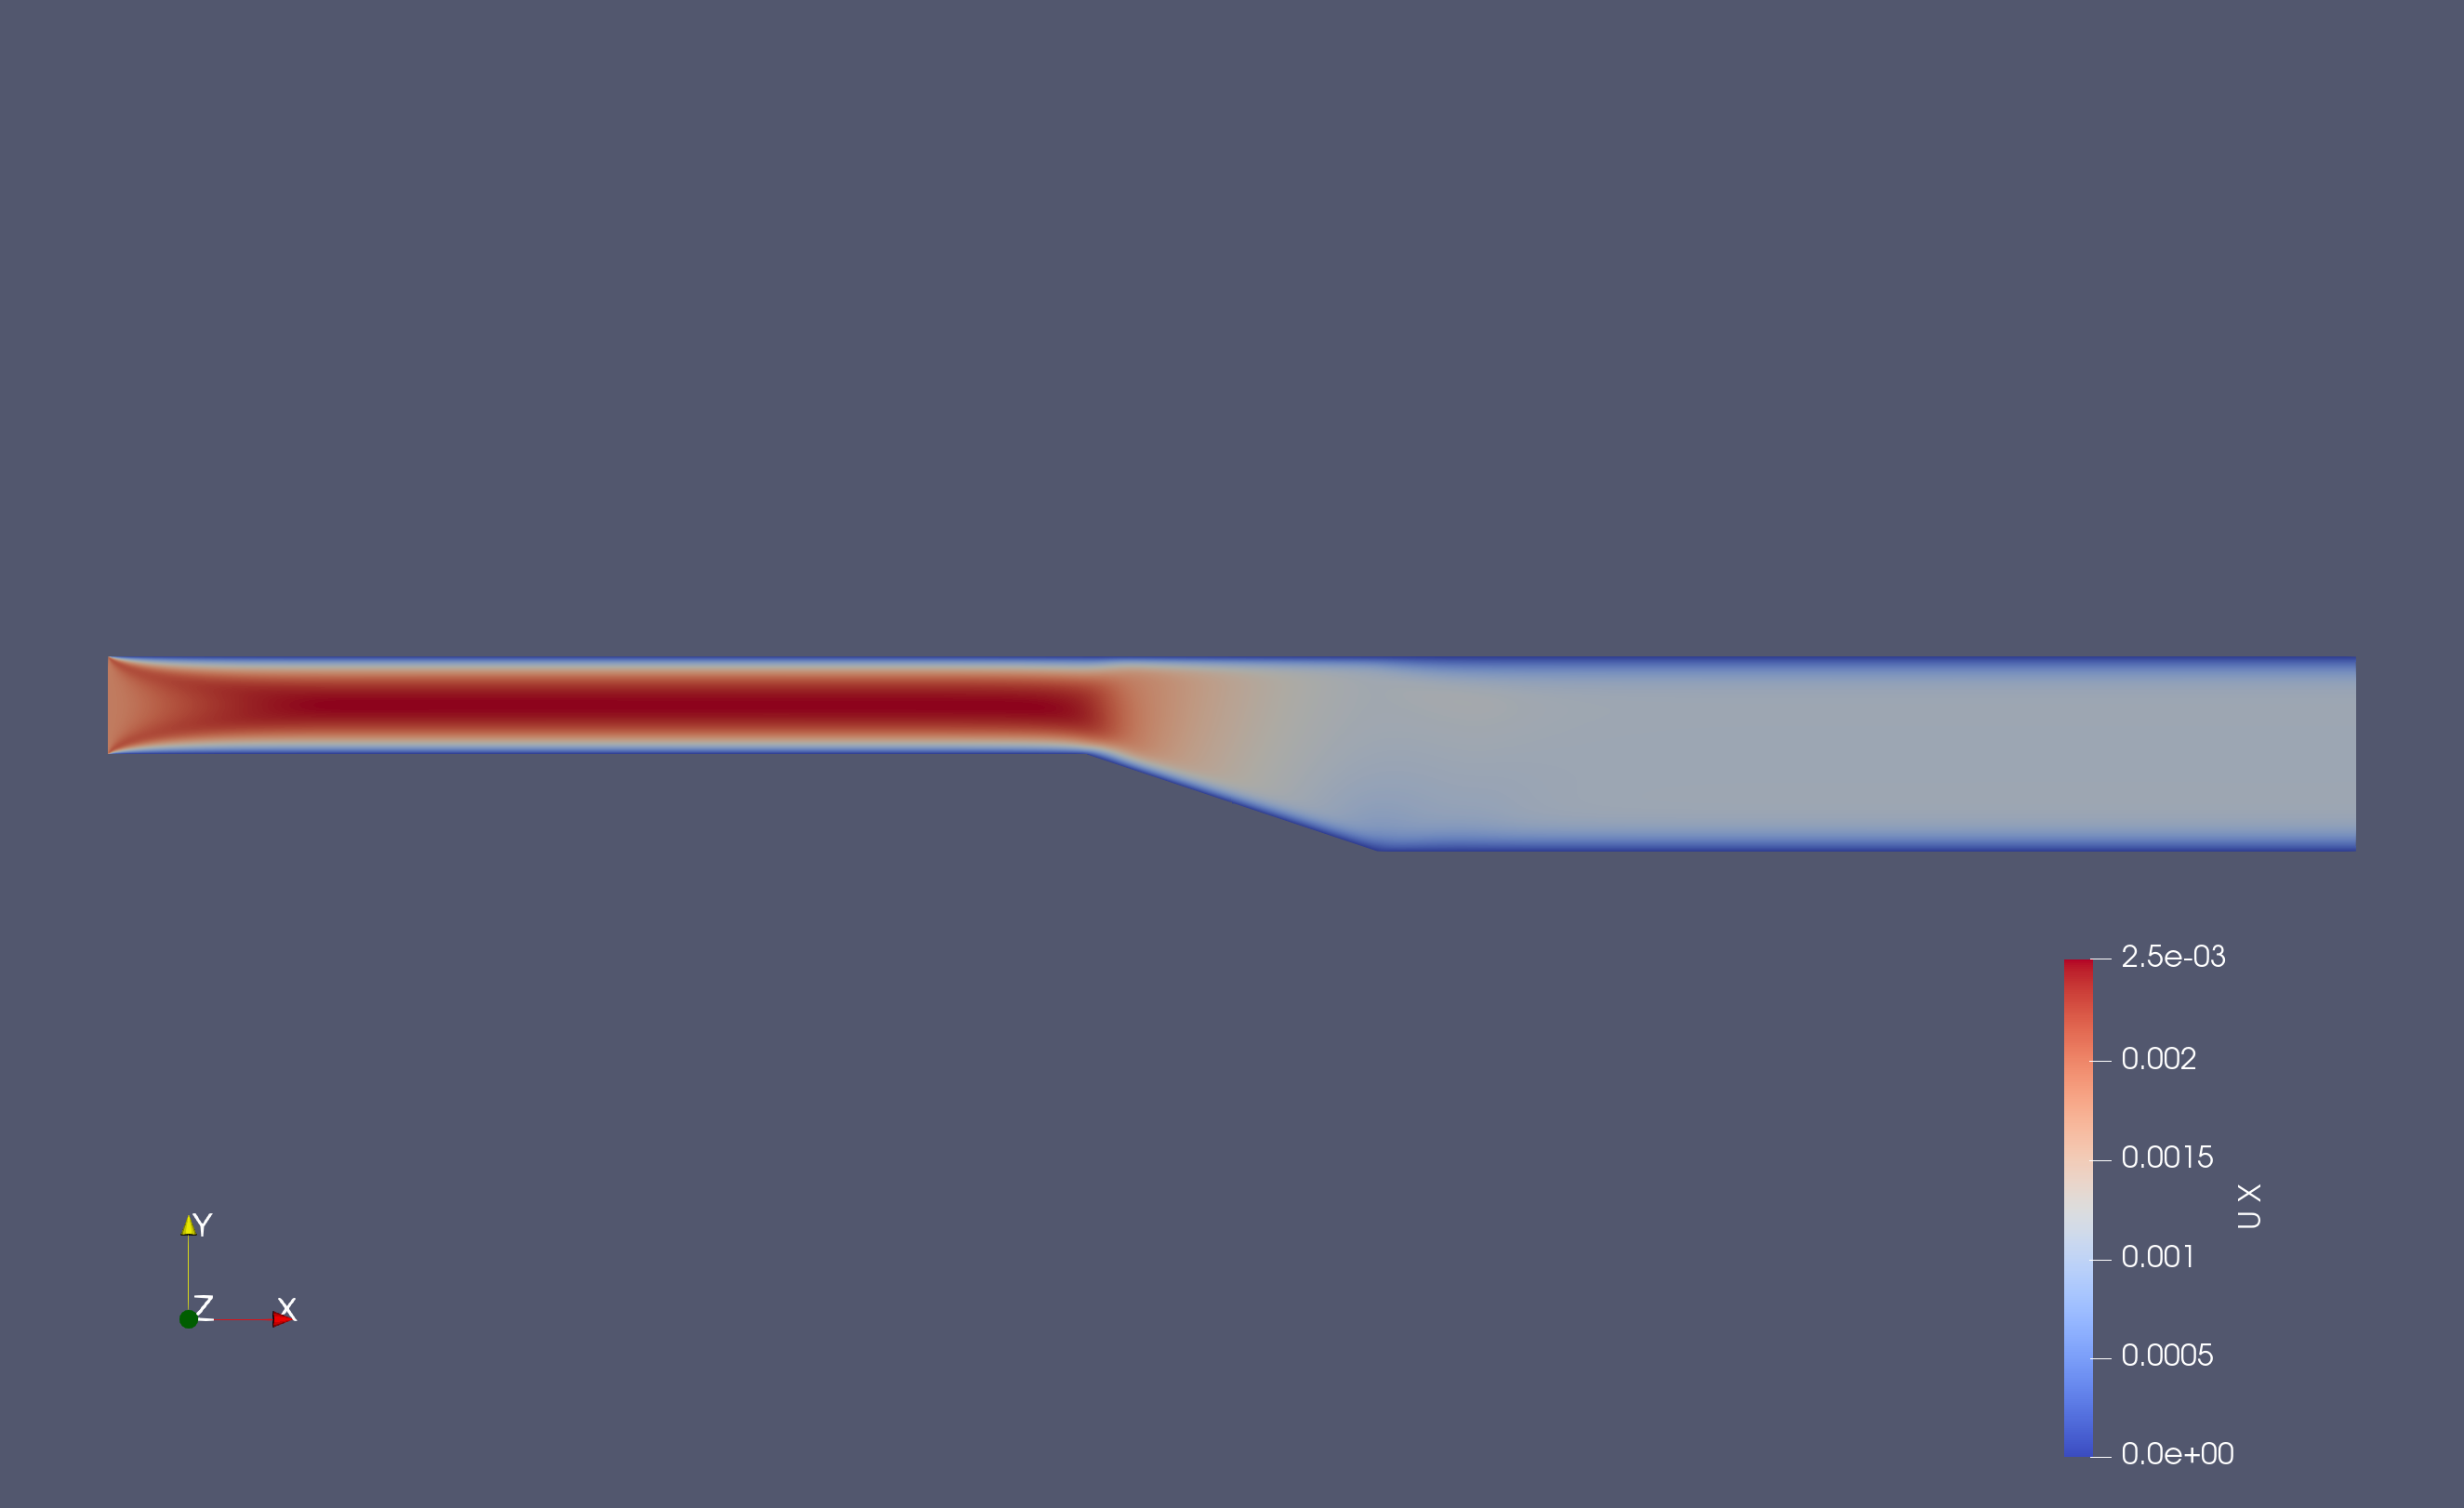
\includegraphics[width=0.5\linewidth]{Imagenes/T1/SimMill.png}
    \caption{$U_x$ del canal simulado de 2.6millones celdas}
    \label{fig:placeholder}
\end{figure}


\newpage
\section{Planteamiento del problema}
\label{sec:problema}

Simulacion de un flujo en un difusor

\subsection{Dominio y geometría}

\begin{figure}[H]
  \centering
  \def\LS{6}   \def\RS{10}   \def\Lr{3}   \def\Hin{1}   \def\Hout{2}
  \resizebox{\textwidth}{!}{%
  \begin{tikzpicture}[
      x=1cm, y=1cm,
      pared/.style   = {line width=1.6pt, line cap=round, line join=round},
      contorno/.style= {line width=0.6pt},
      cota/.style    = {|<->|, >={Latex[length=2mm]}, line width=0.5pt},
      aux/.style     = {line width=0.3pt, densely dashed, gray}
    ]

  % ---- puntos clave ------------------------------------------------
  \pgfmathsetmacro{\xA}{\LS}            % inicio de la rampa
  \pgfmathsetmacro{\xB}{\LS+\Lr}        % fin de la rampa
  \pgfmathsetmacro{\xC}{\LS+\Lr+\RS}    % salida
  \pgfmathsetmacro{\yin}{\Hout-\Hin}    % piso aguas arriba
 
  % ---- paredes solidas (superior e inferior) -----------------------
  \draw[pared] (0,\Hout) -- (\xC,\Hout);
  \draw[pared] (0,\yin) -- (\xA,\yin) -- (\xB,0) -- (\xC,0);
 
  % ---- entrada y salida --------------------------------------------
  \draw[contorno] (0,\yin) -- (0,\Hout);
  \draw[contorno] (\xC,0) -- (\xC,\Hout);
 
  % ---- cotas verticales --------------------------------------------
  \draw[cota] (0.6,\yin) -- (0.6,\Hout)
      node[midway,fill=white,inner sep=1pt] {\SI{1}{\metre}};
  \draw[cota] (\xC-0.8,0) -- (\xC-0.8,\Hout)
      node[midway,fill=white,inner sep=1pt] {\SI{2}{\metre}};
 
  % ---- cotas horizontales (arriba) ---------------------------------
  \draw[aux] (0,\Hout)  -- (0,\Hout+1.4);
  \draw[aux] (\xA,\yin) -- (\xA,\Hout+1.4);
  \draw[aux] (\xB,0)    -- (\xB,\Hout+1.4);
  \draw[aux] (\xC,\Hout)-- (\xC,\Hout+1.4);
 
  \draw[cota] (0,\Hout+1.15)   -- (\xA,\Hout+1.15) node[midway,above] {LS \textit{(leftSide)}};
  \draw[cota] (\xA,\Hout+0.55) -- (\xB,\Hout+0.55) node[midway,above] {\SI{3}{\metre}};
  \draw[cota] (\xB,\Hout+1.15) -- (\xC,\Hout+1.15) node[midway,above] {RS \textit{(rightSide)}};
 
  % ---- caida de la rampa (cota vertical auxiliar) ------------------
  \draw[aux] (\xB,0)    -- (\xB+1.3,0);
  \draw[aux] (\xA,\yin) -- (\xB+1.3,\yin);
  \draw[cota] (\xB+1.1,0) -- (\xB+1.1,\yin)
      node[midway,right,inner sep=2pt] {\SI{1}{\metre}};
 

  \end{tikzpicture}}
  \caption{Dominio computacional, dimensiones características y nomenclatura de
  las fronteras (\archivo{inlet}, \archivo{outlet}, \archivo{leftSide},
  \archivo{rightSide}).}
  \label{fig:dominio}
\end{figure}

\subsection{Propiedades del fluido y parámetros adimensionales}

\begin{table}[H]
  \centering
  \caption{Propiedades físicas y parámetros de la simulación.}
  \label{tab:propiedades}
  \begin{tabular}{llS[table-format=1.3e2]l}
    \toprule
    Parámetro & Símbolo & {Valor} & Unidad \\
    \midrule
    Longitud característica   & $L$      & 1  & \si{\meter} \\
    Velocidad de entrada  & $U_{in}$      & 0.0018440  & \si{\meter\per\second} \\
    Viscosidad cinemática     & $\nu$    & 1.8440e-05 & \si{\meter\squared\per\second} \\
    Densidad                  & $\rho$   & 1.184  & \si{\kilogram\per\meter\cubed} \\
    Número de Reynolds        & \Rey     & 100 & {--} \\
    \bottomrule
  \end{tabular}
\end{table}

\[
  \Rey = \frac{U L}{\nu}
  \qquad\Longrightarrow\qquad
  \Rey = 100 \;\; \text{(régimen laminar)}
\]

\subsection{Supuestos}

Hipótesis adoptadas: flujo incompresible, isotérmico, propiedades constantes, Bidimensional, estacionario, laminar.

% ======================================================================
\section{Procedimiento}
\label{sec:procedimiento}

Estructura del caso en \OF:

\begin{terminal}
caso/
|-- 0/                  # condiciones iniciales y de borde (U, p, k, epsilon...)
|-- constant/
|   |-- transportProperties
|   `-- turbulenceProperties
|   `-- Parametros      #aqui tuve la idea de hacerlo parametrico para que de esa manera si 
|                       #Que cambiar algo se arregle automaticamente, aprovecho de aprender 
`-- system/
    |-- blockMeshDict
    |-- controlDict
    |-- fvSchemes
    `-- fvSolution
\end{terminal}

% ----------------------------------------------------------------------
\subsection{Parametros}
\label{sec:parametros}

Aqui es donde fui a investigar y preguntar a ChatGPT (Claude) por como hacer este tipo de cosas parametricas, y es parecido a crear una libreria en python donde creas un documento, colocas varias cosas y luego solo lo cargas (si use IA pero tambien estuve leyendo el libro en HTML que tienen (no pensaba comprarlo), es increible que funcione tambien para estructuras) de todos modos, me base mucho en el codigo de Clases, pero no me corrio lamentablemente (problemas de compatibilidad con versiones segun la IA)   \url{https://doc.cfd.direct/openfoam/user-guide-v14}

\begin{foamcode}[caption={Extracto de \archivo{system/blockMeshDict}.},label={lst:blockmesh}]
//     #include "${FOAM_CASE}/constant/Parametros"

H       1;                 // altura de entrada [m]
LS      10;                // prerampa[m]
RS      10;                // PostRampa [m]

Hout    #calc "2 * $H";      // altura de salida = 2H [m]
Ldiff   #calc "3 * $H";      // Largo rampa = 3H [m]

Re      100;                  // Reynolds de enunciado
nu      1.8440831253e-05;     // viscosidad cinematica del aire segun CoolProp (25C y 101kPa)
Uin     #calc "$Re * $nu / $H"; // Calculo velocidad de entrada 

// ************************************************************************* //

\end{foamcode}

\subsection{Malla}
\label{sec:malla}

\subsubsection{Generación}

Aqui basicamente lo que hago es colocar los puntos clave, que son 4 coordenadas en x, inicio, inicio rampa, termino rampa, termino todo, esos son funcion del largo rampa, mas largo antes y post rampa., los puntos y clave son  

\begin{foamcode}[caption={Extracto de \archivo{system/blockMeshDict}.},label={lst:blockmesh}]
#include "${FOAM_CASE}/constant/Parametros"
// Lo que hago es colocar todos los puntos clave
zBack   #calc "0.1 * $H";   // espesor en z (caso 2D) [m]

x0      0;
x1      $LS;
x2      #calc "$LS + $Ldiff";
x3      #calc "$LS + $Ldiff + $RS";

yTop    $Hout;                // tecgo superior
y0In    #calc "$Hout - $H";   // suelo mitad
y0Out   0;                    // suelo inferior

z0      0;
z1      $zBack;   //Simplemente tomo el ancho
//Aqui vienen las divisiones
dx      #calc "$H / 10.0";  // arriba y abajo
dxDiff  #calc "$H / 20.0";  // rampa donde tengo malla mas fina

nx1     #calc "label(round($LS / $dx))";       // celdas 1
nx2     #calc "label(round($Ldiff / $dxDiff))"; // celdas 2
nx3     #calc "label(round($RS / $dx))";       // celdas 3
ny      60;     // en y igual para buena continuidad "ni idea pero si cambio me tiraba problemas"
nz      1;      // celdas en z (caso 2D)
// Refinamiento hacia el techo y el piso
yGrading simpleGrading (1 ((0.5 0.5 4)(0.5 0.5 0.25)) 1);

//Me salto los vertices para que no quede muy largo pero es bastante explicatorio las combinaciones
blocks
(
    hex (0 4 6 2 1 5 7 3)       ($nx1 $ny $nz) $yGrading
    hex (4 8 10 6 5 9 11 7)     ($nx2 $ny $nz) $yGrading
    hex (8 12 14 10 9 13 15 11) ($nx3 $ny $nz) $yGrading
);

\end{foamcode}
Ahora corro los siguientes formatos que me generan la malla, y la puedo checkera que este todo bien

\begin{terminal}
blockMesh
checkMesh
\end{terminal}
Que maravillosa es la IA para poder pasar de codigo feo a bonitas figuras en tikz, coloco este bloque para que se entienda como fue la division general, cada nodo con su numero de nodo, tambienm como uni los nodos entre ellos
\begin{figure}[!ht]
    \centering
 %---- proporciones del esquema (no a escala real, solo ilustrativo) ----
\def\XA{4}      % x1 = LS
\def\XB{7}      % x2 = LS + Ldiff
\def\XC{12}     % x3 = LS + Ldiff + RS
\def\YT{2}      % yTop  = Hout
\def\YI{1}      % y0In  = Hout - H
\def\YO{0}      % y0Out = 0
\def\DX{1.0}    % desplazamiento visual de z1 (eje z)
\def\DY{0.7}
 
\begin{tikzpicture}[
    x=1cm, y=1cm,
    front/.style  = {line width=1.2pt, line join=round},
    back/.style   = {line width=0.5pt, gray, densely dashed, line join=round},
    link/.style   = {line width=0.4pt, gray, densely dotted},
    divi/.style   = {line width=0.5pt, densely dashed},
    vf/.style     = {circle, draw, fill=white, inner sep=0.9pt, font=\tiny},
    vb/.style     = {circle, draw=gray, fill=white, inner sep=0.9pt,
                     font=\tiny, text=gray},
    flecha/.style = {arrows={-Latex[length=1.8mm]}, line width=0.6pt},
    rot/.style    = {font=\footnotesize},
    bloque/.style = {draw, rounded corners=1pt, inner sep=2pt,
                     font=\footnotesize\bfseries, fill=white},
    cota/.style   = {arrows={Bar[]Latex[length=2mm]-Latex[length=2mm]Bar[]},
                     line width=0.5pt}
  ]
 
  % ================= plano trasero  z = z1 =========================
  \begin{scope}[shift={(\DX,\DY)}]
    \draw[back] (0,\YI) -- (\XA,\YI) -- (\XB,\YO) -- (\XC,\YO)
                -- (\XC,\YT) -- (0,\YT) -- cycle;
    \draw[back] (\XA,\YI) -- (\XA,\YT);
    \draw[back] (\XB,\YO) -- (\XB,\YT);
  \end{scope}
 
  % ================= aristas que unen z0 con z1 ====================
  \foreach \p in {(0,\YI),(0,\YT),(\XA,\YI),(\XA,\YT),
                  (\XB,\YO),(\XB,\YT),(\XC,\YO),(\XC,\YT)}
    {\draw[link] \p -- ++(\DX,\DY);}
 
  % ================= plano frontal  z = z0 =========================
  \draw[front] (0,\YI) -- (\XA,\YI) -- (\XB,\YO) -- (\XC,\YO)
               -- (\XC,\YT) -- (0,\YT) -- cycle;
  \draw[divi] (\XA,\YI) -- (\XA,\YT);
  \draw[divi] (\XB,\YO) -- (\XB,\YT);
 
  % ================= sentido de giro del bloque 1 ==================
  \draw[flecha] (0.55,\YI+0.18) -- (\XA-0.55,\YI+0.18);      % 0 -> 4
  \draw[flecha] (\XA-0.18,\YI+0.35) -- (\XA-0.18,\YT-0.35);  % 4 -> 6
  \draw[flecha] (\XA-0.55,\YT-0.18) -- (0.55,\YT-0.18);      % 6 -> 2
  \draw[flecha] (0.18,\YT-0.35) -- (0.18,\YI+0.35);          % 2 -> 0
 
  % ================= vertices del plano z1 =========================
  \node[vb] at (0+\DX,\YI+\DY)    {1};
  \node[vb] at (0+\DX,\YT+\DY)    {3};
  \node[vb] at (\XA+\DX,\YI+\DY)  {5};
  \node[vb] at (\XA+\DX,\YT+\DY)  {7};
  \node[vb] at (\XB+\DX,\YO+\DY)  {9};
  \node[vb] at (\XB+\DX,\YT+\DY) {11};
  \node[vb] at (\XC+\DX,\YO+\DY) {13};
  \node[vb] at (\XC+\DX,\YT+\DY) {15};
 
  % ================= vertices del plano z0 =========================
  \node[vf] at (0,\YI)    {0};
  \node[vf] at (0,\YT)    {2};
  \node[vf] at (\XA,\YI)  {4};
  \node[vf] at (\XA,\YT)  {6};
  \node[vf] at (\XB,\YO)  {8};
  \node[vf] at (\XB,\YT) {10};
  \node[vf] at (\XC,\YO) {12};
  \node[vf] at (\XC,\YT) {14};
 
  % ================= identificador de cada bloque ==================
  \node[bloque] at ({\XA/2},{(\YI+\YT)/2})        {1};
  \node[bloque] at ({(\XA+\XB)/2},{\YT-0.85})     {2};
  \node[bloque] at ({(\XB+\XC)/2},{\YT/2})        {3};
 
  % ================= nombres de las fronteras ======================
  \node[rot,rotate=90,anchor=south] at (-0.40,{(\YI+\YT)/2}) {\texttt{inlet}};
  \node[rot,rotate=90,anchor=north] at (\XC+0.40,{(\YO+\YT)/2}) {\texttt{outlet}};
  \node[rot,anchor=north] at (\XB,\YO-0.30) {\texttt{lowerWall}};
  \node[rot,anchor=center] at (9.6,{\YT+0.36}) {\texttt{upperWall}};
  \node[rot,anchor=south west,gray] at (3.6,{\YT+\DY+0.18})
    {\texttt{frontAndBack} (\texttt{empty}): las dos caras $x$--$y$};
 
  % ================= coordenadas ===================================
  \begin{scope}[shift={(0,-1.55)}]
    \draw[flecha] (0,0) -- (1.1,0)     node[right,rot] {$x$};
    \draw[flecha] (0,0) -- (0,0.9)     node[above,rot] {$y$};
    \draw[flecha] (0,0) -- (0.62,0.43) node[right,rot,xshift=1pt] {$z$};
  \end{scope}
 
  % ================= leyenda =======================================
 
  % ================= cotas en x ====================================
  \draw[cota] (0,-3.5) -- (\XA,-3.5) node[midway,fill=white,inner sep=1pt,rot]
    {\texttt{x0}--\texttt{x1}: $LS$};
  \draw[cota] (\XA,-3.5) -- (\XB,-3.5) node[midway,fill=white,inner sep=1pt,rot]
    {$3H$};
  \draw[cota] (\XB,-3.5) -- (\XC,-3.5) node[midway,fill=white,inner sep=1pt,rot]
    {\texttt{x2}--\texttt{x3}: $RS$};
 
\end{tikzpicture}

    \caption{Caption}
    \label{fig:placeholder}
\end{figure}
\subsubsection{Calidad de la malla}

Resumen de la salida de \comando{checkMesh}:

\begin{table}[H]
  \centering
  \caption{Métricas de calidad reportadas por \comando{checkMesh}.}
  \label{tab:checkmesh}
  \begin{tabular}{lS[table-format=5.3]l}
    \toprule
    Métrica & {Valor} & Criterio \\
    \midrule
    N.º de celdas            & 15600  & {--} \\
    Máxima no ortogonalidad  & 18.369  & OK\\
    Máximo \emph{skewness}   & 0.367  & OK \\
    Máxima razón de aspecto  & 13.0538   & OK \\
    \midrule
    \multicolumn{3}{l}{\textbf{Mesh OK.} asi que god} \\
    \bottomrule
  \end{tabular}
\end{table}

\begin{figure}[H]
  \centering
  \begin{subfigure}[b]{0.47\textwidth}
    \centering
    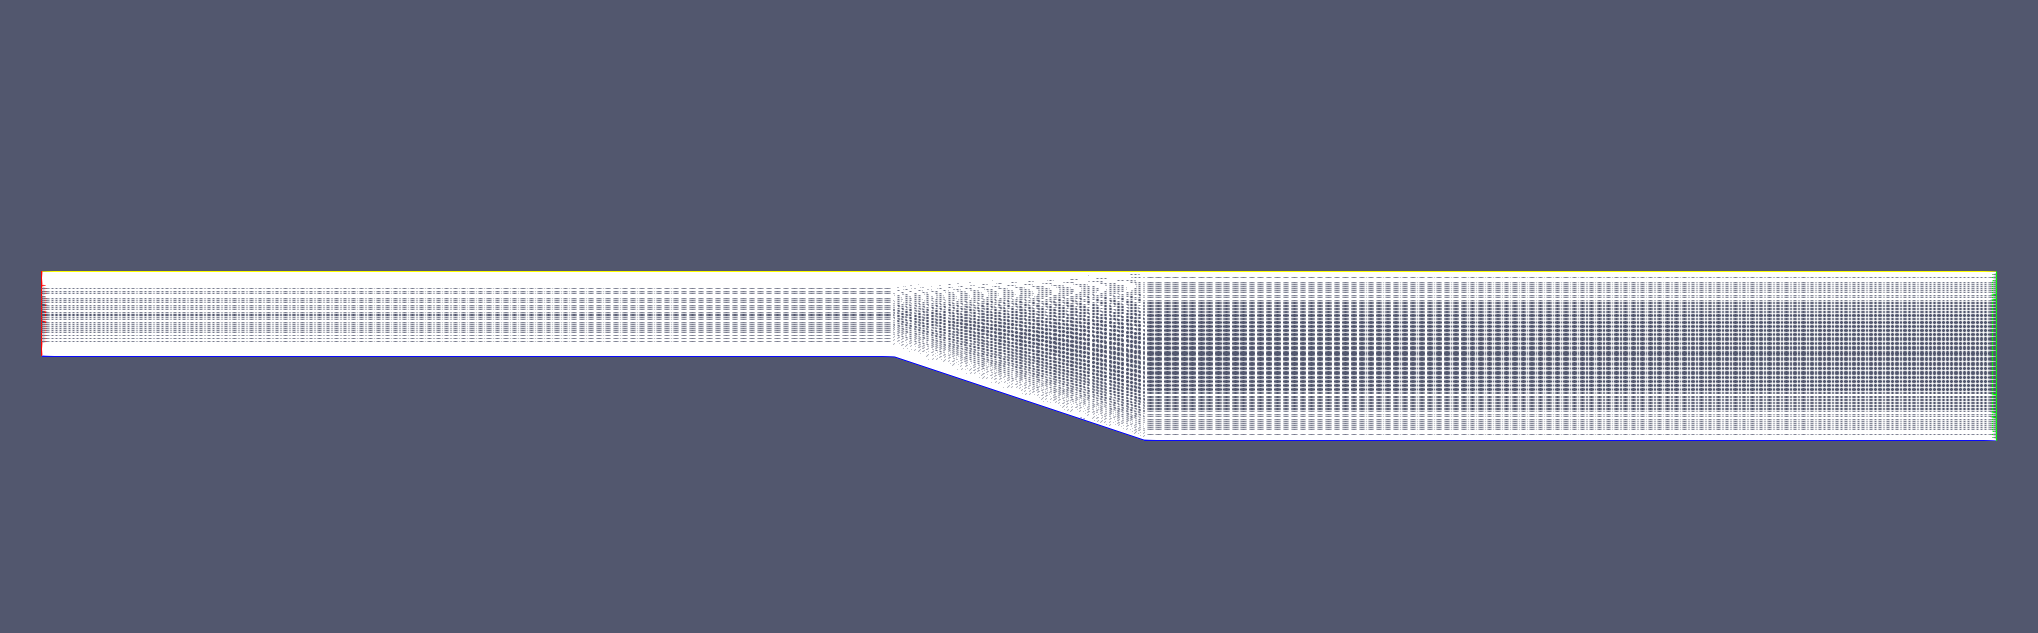
\includegraphics[width=\textwidth]{Imagenes/T1/malla_global.png}

    \caption{Vista global.}
  \end{subfigure}\hfill
  \begin{subfigure}[b]{0.47\textwidth}
    \centering
    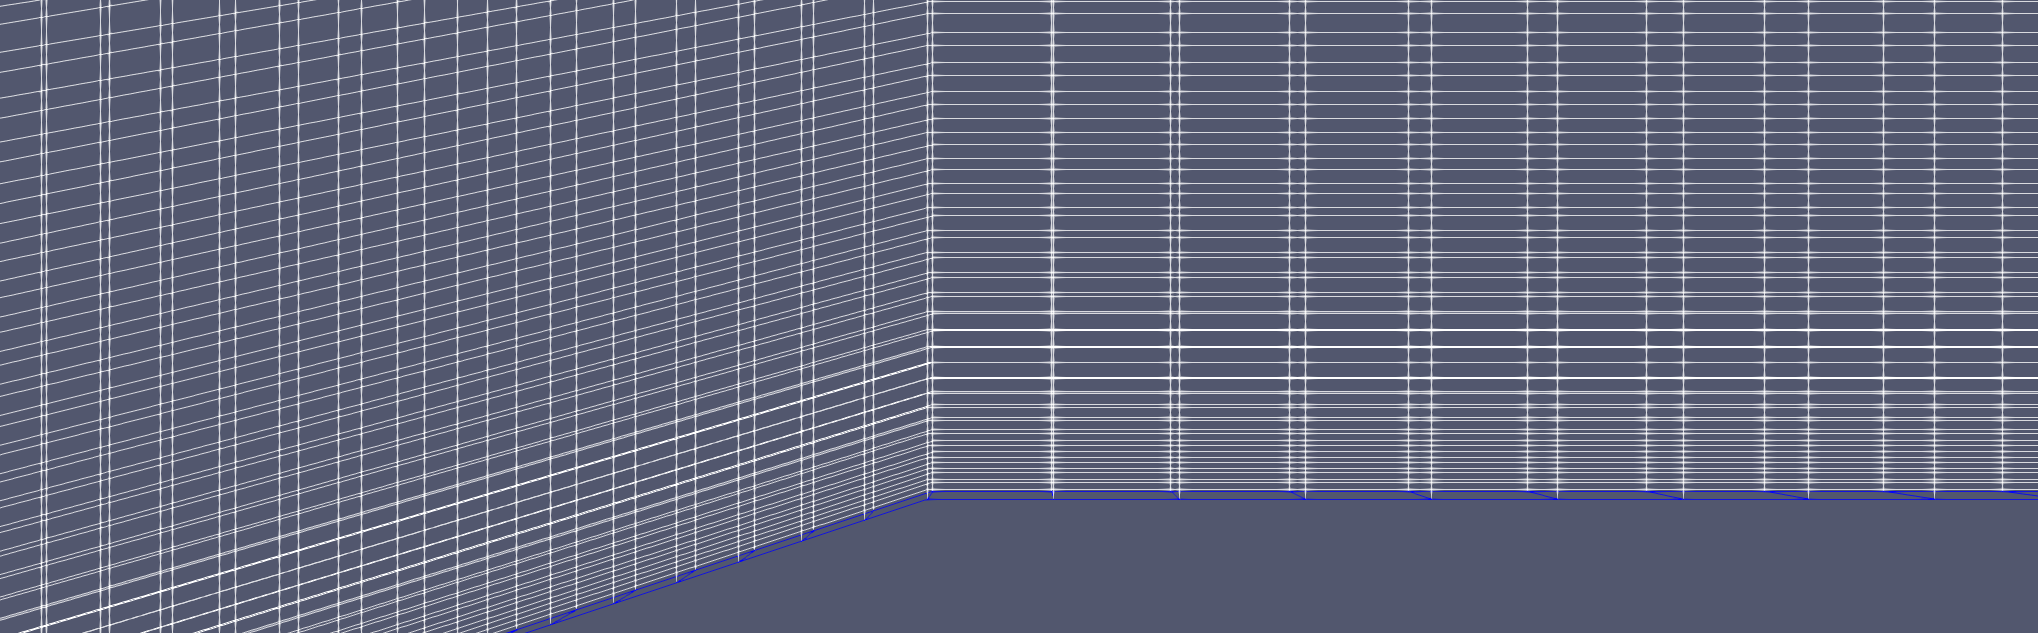
\includegraphics[width=\textwidth]{Imagenes/T1/malla_detalle.png}
    \caption{Detalle del refinamiento en la pared.}
  \end{subfigure}
  \caption{Malla generada con \comando{blockMesh}.}
  \label{fig:malla}
\end{figure}

\subsubsection{Independencia de malla}

\begin{table}[H]
  \centering
  \caption{Estudio de independencia de malla. La variable de control es la velocidad máxima del perfil antes de la rampa}
  \label{tab:independencia}
  \begin{tabular}{lS[table-format=6.0]S[table-format=2.4]S[table-format=2.2]}
    \toprule
    Malla & {Celdas} & {Variable de control} \\
    \midrule
    Gruesa & 2600   & 0.0027  \\
    Media  & 15600 & 0.0025  \\
    Fina   & 33000  & 0.0025  \\
    ultrafina  & 2.6mill & 0.0025  \\
    \bottomrule
  \end{tabular}
\end{table}

Se considera convergida la malla cuando la variación de la
velocidad entre niveles sucesivos es indistinguible a 2 cifras significativas, con esto llegamos a que pasado los 15600 celdas estamos bien.

% ----------------------------------------------------------------------
\subsection{Condiciones iniciales y de borde}
\label{sec:condiciones}

\subsubsection{Resumen de condiciones}

\begin{table}[H]
  \centering
  \caption{Condiciones de borde impuestas en la carpeta \archivo{0/}.}
  \label{tab:condiciones}
  \begin{tabular}{lll}
    \toprule
    Frontera & $\vect{u}$ (\archivo{0/U}) & $p$ (\archivo{0/p}) \\
    \midrule
    \archivo{Inlet}   & \archivo{fixedValue}, $(-U_{in}\;0\;0)$ & \archivo{zeroGradient} \\
    \archivo{Outlet}   & \archivo{zeroGradient} & \archivo{fixedValue}, $0$ \\
    \archivo{"(lowerWall|upperWall)"}   & \archivo{noSlip}                  & \archivo{zeroGradient} \\
    \archivo{frontAndBack} & \archivo{empty}                   & \archivo{empty} \\
    \bottomrule
  \end{tabular}
\end{table}
De esta manera le doy una velocidad inicial a la entrada de  $U_{in}$, en las paredes la condicion de no deslizamiento, aparte en presion no hay gradiente hacia las paredes. en el caso de Inlet tengo en presión \archivo{zeroGradient}, esto es debido a que para SIMPLE no es bueno sobre determinar el sistema, debo dejar variables libres. 


\subsubsection{Propiedades de transporte }

\begin{foamcode}[caption={\archivo{constant/transportProperties} y \archivo{constant/turbulenceProperties}.}]
nu              [0 2 -1 0 0 0 0] 1.8440831253e-05; // De CoolProp 25grados 101,3kPa

simulationType  laminar;
\end{foamcode}

% ----------------------------------------------------------------------
\subsection{Configuración numérica}
Personalmente no tengo mucha idea de como funciona, pero colocare lo que entendi, es como trabaja con las derivadas, por ejemplo las temporales deben ser 0 por eso, grad es el gradiente asi.

\label{sec:numerica}

\begin{table}[H]
  \centering
  \caption{Esquemas de discretización (\archivo{system/fvSchemes}).}
  \label{tab:schemes}
  \begin{tabular}{ll}
    \toprule
    Término & Esquema\\
    \midrule
    \archivo{ddtSchemes}        & \archivo{steadyState}  \\
    \archivo{gradSchemes}       & \archivo{Gauss linear}    \\
    \archivo{divSchemes}        & \archivo{Gauss linearUpwind}  \\
    \archivo{laplacianSchemes}  & \archivo{Gauss linear corrected} \\
    \bottomrule
  \end{tabular}
\end{table}
Luego simplemente correr la simulación, una vez tenga eso tambien corri un codigo que me tomaba lo datos y de daba un csv para poder analkizarlo con python 
\begin{terminal}
    /*--------------------------------*- C++ -*----------------------------------*\
  =========                 |
  \\      /  F ield         | OpenFOAM: The Open Source CFD Toolbox
   \\    /   O peration     | Website:  https://openfoam.org
    \\  /    A nd           | Version:  14
     \\/     M anipulation  |
\*---------------------------------------------------------------------------*/
FoamFile
{
    format      ascii;
    class       dictionary;
    object      sampleDict;
}
// * * * * * * * * * * * * * * * * * * * * * * * * * * * * * * * * * * * * * //
// Lineas de muestreo de U en la seccion de entrada y de salida, para
// comparar contra la solucion analitica de Poiseuille plano.
//
// Posiciones (parametrizadas con distOffset, en metros):
//   - aguas arriba: distOffset despues del comienzo del dominio (x0 = 0)
//   - aguas abajo : distOffset antes del final del dominio (x3 = LS+Ldiff+RS)

#include "${FOAM_CASE}/constant/Parametros"

distOffset  1;                                          // separacion desde cada extremo [m]

xInlet      #calc "0 + $distOffset";                     // seccion de entrada (tramo recto izq.)
xOutlet     #calc "$LS + $Ldiff + $RS - $distOffset";     // seccion de salida (tramo recto der.)

zMid        #calc "0.05 * $H";   // plano medio en z (zBack = 0.1*H en blockMeshDict)

y0In        #calc "$Hout - $H";  // pared inferior en el tramo de entrada (= H)
y0Out       0;                   // pared inferior en el tramo de salida
yTop        $Hout;               // pared superior, constante en todo el dominio

type            sets;
libs            ("libsampling.so");
interpolationScheme cellPoint;
setFormat       raw;

sets
(
    inletProfile
    {
        type    lineUniform;
        axis    y;
        start   ($xInlet $y0In $zMid);
        end     ($xInlet $yTop $zMid);
        nPoints 200;
    }
    outletProfile
    {
        type    lineUniform;
        axis    y;
        start   ($xOutlet $y0Out $zMid);
        end     ($xOutlet $yTop  $zMid);
        nPoints 200;
    }
);

fields (U);

// ************************************************************************* //

\end{terminal}
% ======================================================================
\section{Resultados}
\label{sec:resultados}

\subsection{Influencia del dominio computacional}
En este caso lo haré mediante mediciones del perfil de velocidades, por teoria se supone que esto sigue un flujo de Poiseuille plano el cual ya esta resuelto, por ende mediante ecuaciones puedo llegar al perfil teórico antes y después del difusor, tomare una medida de error y un umbral.

\subsection{Caudal a partir del perfil simulado}
En cada sección, el caudal simulado por unidad de profundidad se calcula por
la integral del perfil extraído:
\[
Q_{\text{sim}} = \int_0^{H_{\text{local}}} u_{\text{sim}}(y)\,dy .
\]

\subsection{Perfil teórico equivalente}
Para cada sección se construye el perfil teórico de Poiseuille plano usando
el caudal medido en la misma sección y su altura local
($H_{\text{local}}=H$ en la entrada, $2H$ en la salida):
\[
u_{\text{teo}}(y) = \frac{6\,Q_{\text{sim}}}{H_{\text{local}}^3}\, y\,(H_{\text{local}}-y).
\]

Al usar el caudal propio de cada sección, la comparación aísla si la
forma del perfil simulado corresponde a Poiseuille plano,
independientemente del balance global de masa.
Tener en cuenta que esto no tiene en cuenta perdidas de energia por distintos factores por ende puede variar, por eso tomamos el error/umbral de 5\% 
el error relativo al teorico |
\[
e_{\text{rel}} = \frac{\lVert u_{\text{sim}} - u_{\text{teo}} \rVert_2}
                       {\lVert u_{\text{teo}} \rVert_2}\]


\newpage
\subsubsection{Aguas arriba}
Para analizar aguas arriba, es mas que nada en que punto se asemeja al perfil real, por ende corrí varios metros y mire el perfil hasta que estabilice\\
\begin{figure}[!ht]
    \centering
    \begin{subfigure}[b]{0.48\linewidth}
        \centering
        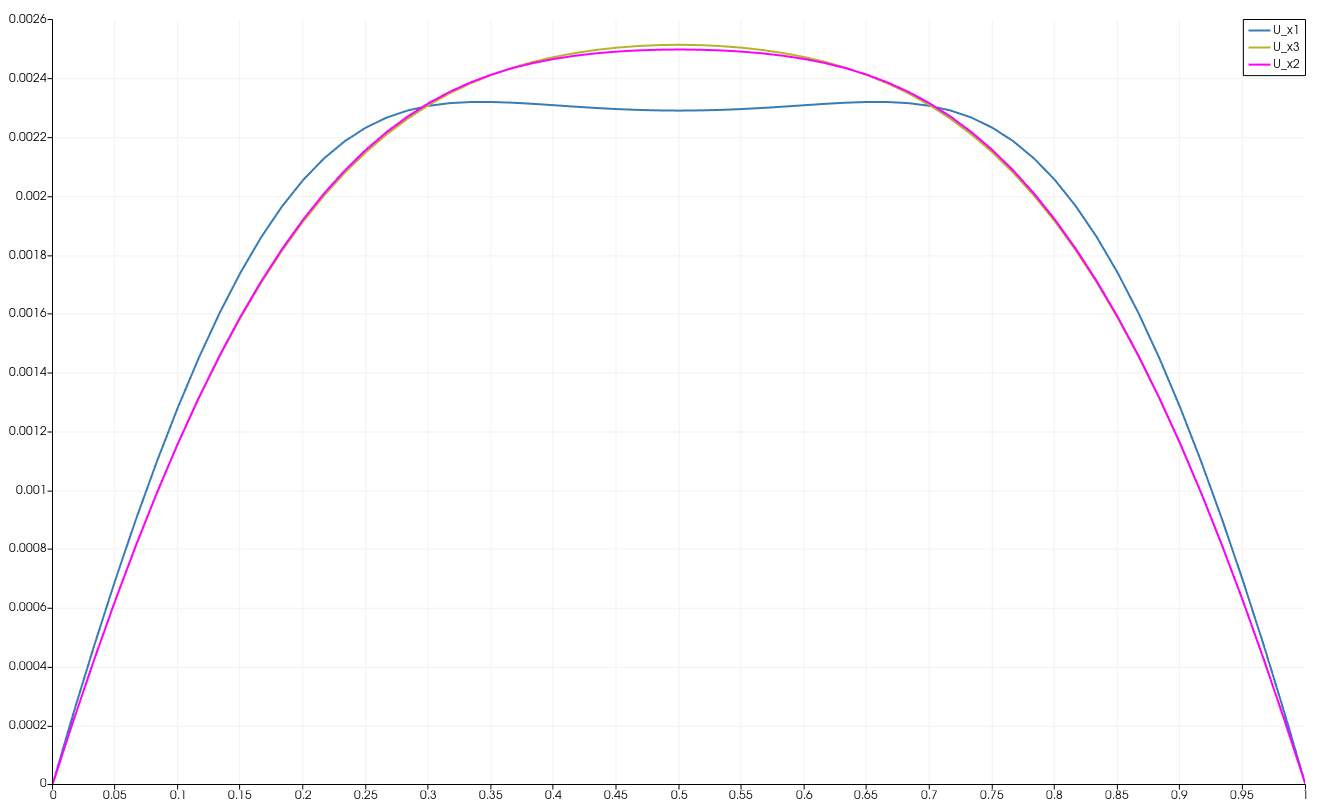
\includegraphics[width=\linewidth]{Imagenes/T1/pArriba123.png}
        \caption{Perfil de velocidad $U_x$ a 1, 2 y 3 metros}
        \label{fig:agua_arriba_123}
    \end{subfigure}
    \hfill
    \begin{subfigure}[b]{0.48\linewidth}
        \centering
        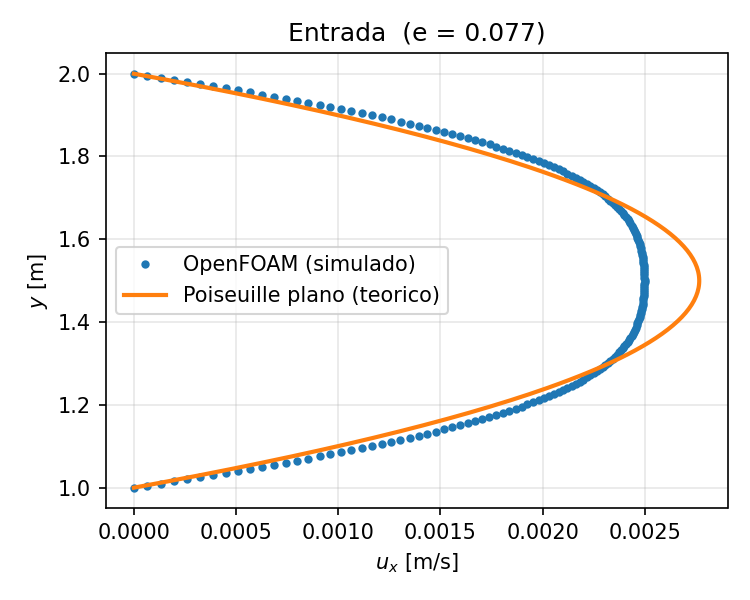
\includegraphics[width=\linewidth]{Imagenes/T1/perfil_entrada.png}
        \caption{Perfil de velocidad $U_x$ a 2 metros comparado con el teórico (error 7.7\%)}
        \label{fig:agua_arriba_teorico}
    \end{subfigure}
    \caption{Comparación de perfiles de velocidad en la sección de entrada}
    \label{fig:agua_arriba}
\end{figure}
Como se puede apreciar ya en 2 metros no hay diferencia notoria con 3 metros, lo que si bastante distinto de Poiseuille
Corri con algunos $x$ mas este error y tendia a cerrar en 7.4\%
\vspace{1cm}
\subsubsection{Aguas Abajo}
Aqui pude hacer lo mismo
\begin{figure}[!ht]
    \centering
    \begin{subfigure}[b]{0.48\linewidth}
        \centering
        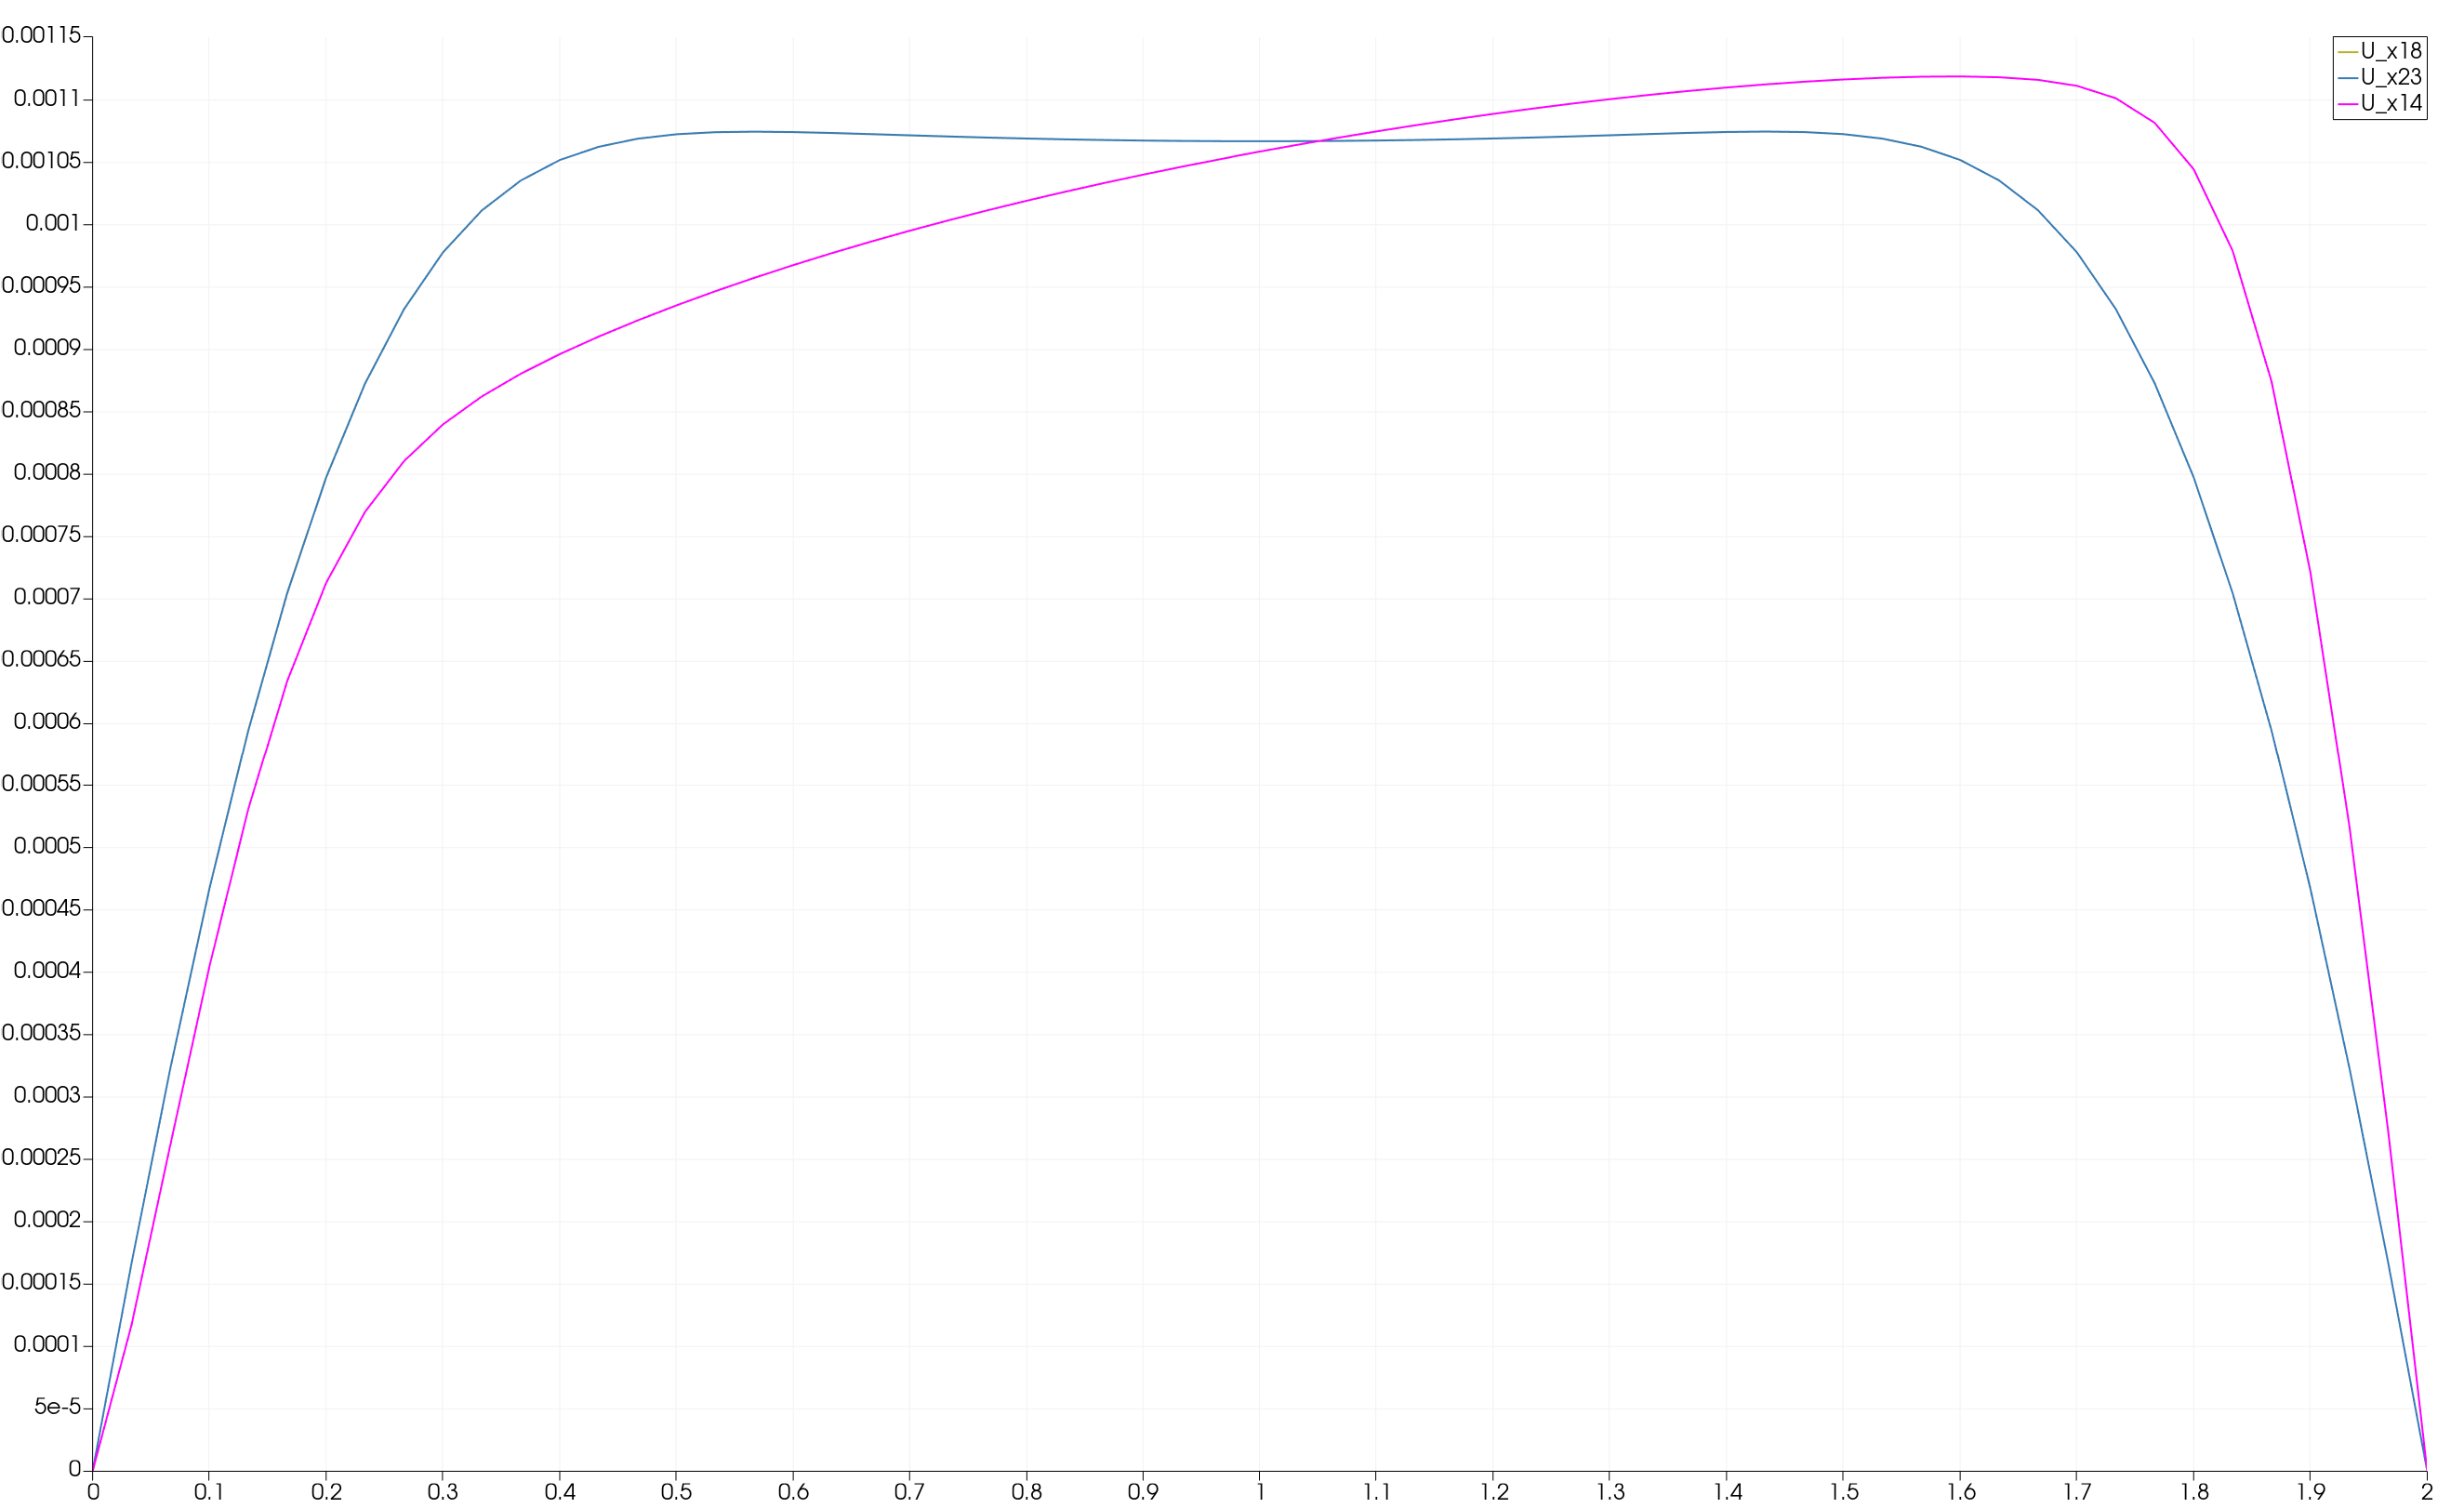
\includegraphics[width=\linewidth]{Imagenes/T1/pAbajo123.png}
        \caption{Perfil de velocidad $U_x$ a 14, 18 y 23 metros}
        \label{fig:agua_arriba_123}
    \end{subfigure}
    \hfill
    \begin{subfigure}[b]{0.48\linewidth}
        \centering
        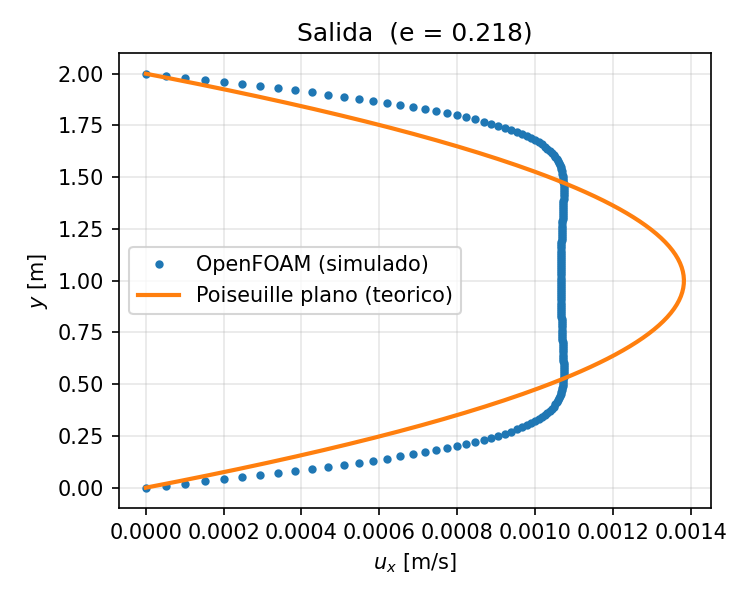
\includegraphics[width=\linewidth]{Imagenes/T1/perfil_salida.png}
        \caption{Perfil de velocidad $U_x$ a 10 metros post pendiente  comparado con el teórico (error 21.8\%)}
        \label{fig:agua_arriba_teorico}
    \end{subfigure}
    \caption{Comparación de perfiles de velocidad en la sección de salida}
    \label{fig:agua_arriba}
\end{figure}
Como se aprecia, pasado los 5 metros desde la rampa no mayor diferencia.

\subsection{Influencia Dominio}
Una vez vi que existe poco cambio pasado los 3 Metros aguas arriba y pasados los 8 metros aguas abajo, corri 24 simulaciones, las cuales son todas las combinaciones de ellas obtuve información que aguas arriba el dominio  no cambia mucho despues de los 2 metros, en cambio aguas abajo si cambiaba mucho mas, en especial la condicion de presion, ya que obliga al final del canal a llegar a 0, en casos puede llegar a que esta presion no vuelva a subir como si lo hace si se deja dentro del dominio computacional, también con simulaciones muy largas, se tiene que hay partes del fluido que son muy similares. Para mas info revisar resumen es bastante bueno explicando todo eso.






\newpage
\section{Anexo}
\begin{figure}[!ht]
    \centering
    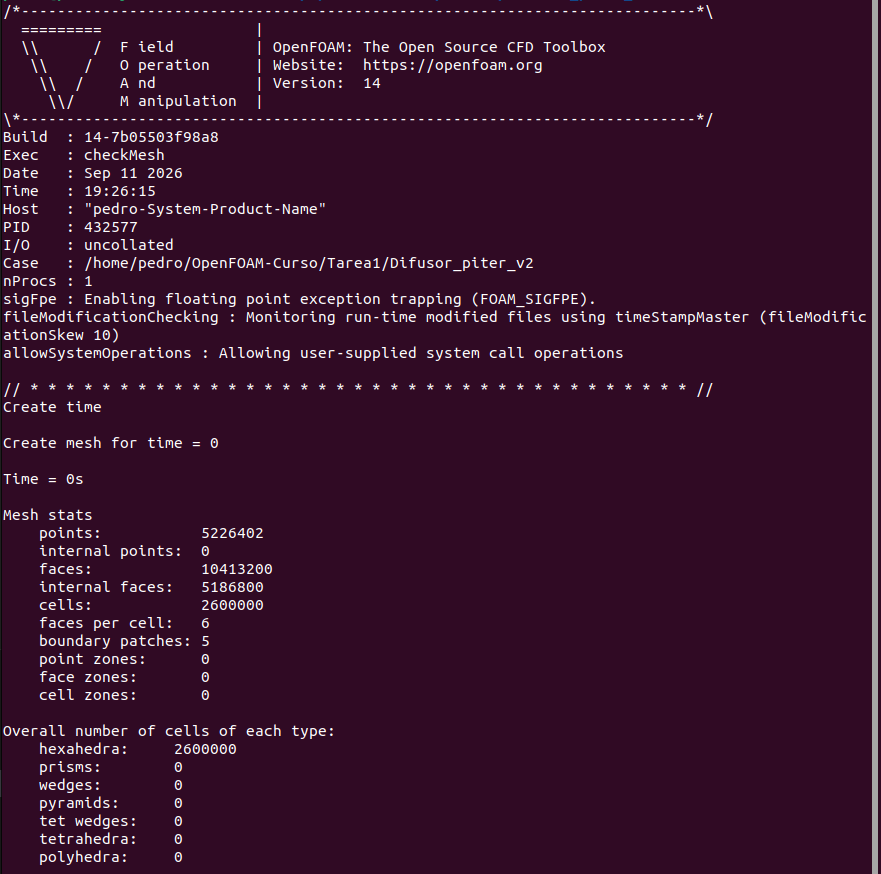
\includegraphics[width=0.75\linewidth]{2.6millones de celdas.png}
    \caption{CheckMesh de simulacion muy muy fina}
    \label{fig:placeholder}
\end{figure}

\begin{terminal}
    Create time

Create mesh for time = 0

Time = 0s

Mesh stats
    points:           5226402
    internal points:  0
    faces:            10413200
    internal faces:   5186800
    cells:            2600000
    faces per cell:   6
    boundary patches: 5
    point zones:      0
    face zones:       0
    cell zones:       0

Overall number of cells of each type:
    hexahedra:     2600000
    prisms:        0
    wedges:        0
    pyramids:      0
    tet wedges:    0
    tetrahedra:    0
    polyhedra:     0

Checking topology...
    Boundary definition OK.
    Cell to face addressing OK.
    Point usage OK.
    Upper triangular ordering OK.
    Face vertices OK.
    Number of regions: 1 (OK).

Checking patch topology for multiply connected surfaces...
    Patch               Faces    Points   Surface topology                  
    inlet               200      402      ok (non-closed singly connected)  
    outlet              200      402      ok (non-closed singly connected)  
    lowerWall           13000    26002    ok (non-closed singly connected)  
    upperWall           13000    26002    ok (non-closed singly connected)  
    frontAndBack        5200000  5226402  ok (non-closed singly connected)  

Checking geometry...
    Overall domain bounding box (0 0 0) (23 2 0.1)
    Mesh has 2 geometric (non-empty/wedge) directions (1 1 0)
    Mesh has 2 solution (non-empty) directions (1 1 0)
    All edges aligned with or perpendicular to non-empty directions.
    Max cell openness = 2.75822e-16 OK.
    Max aspect ratio = 18.6216 OK.
    Minimum face area = 2.30726e-06. Maximum face area = 0.0018455.  Face area magnitudes OK.
    Min volume = 2.30726e-07. Max volume = 3.691e-06.  Total volume = 3.45.  Cell volumes OK.
    Mesh non-orthogonality Max: 18.4151 average: 5.3842
    Non-orthogonality check OK.
    Face pyramids OK.
    Max skewness = 0.833317 OK.
    Coupled point location match (average 0) OK.

Mesh OK.


\end{terminal}


\section{Uso ia}
Para esta entrega se uso IA, en la generacion de codigo de openFOAM (generacion de nodos paramétricos(pasar de nodos a mano a parametricos), explicacion sobre solvers, sobre que hace cada cosa de los codigos, sobre errores, generacion de codigo para tomar valores (perfiles) de las simulaciones), python (creacion de codigo para graficar esos perfiles que saque antes con OpenFoam), Generacion de codigo Tikz y de esta planilla (las palabras dentro de ella son mias probablemente vea faltas de ortografia, y ideas locas son mias), 